% =====================================================================
% schema_newton_cg.tex — Schema Newton-CG, fig:newton_cg della tesi
% Stesso codice TikZ della tesi; compilare con pdflatex.
% =====================================================================
\documentclass[border=8pt]{standalone}
\usepackage[T1]{fontenc}
\usepackage[utf8]{inputenc}
\usepackage{amsmath, amssymb}
\usepackage{tikz}
\usetikzlibrary{arrows.meta, positioning, calc}
\definecolor{coverblue}{RGB}{30, 60, 120}

\begin{document}
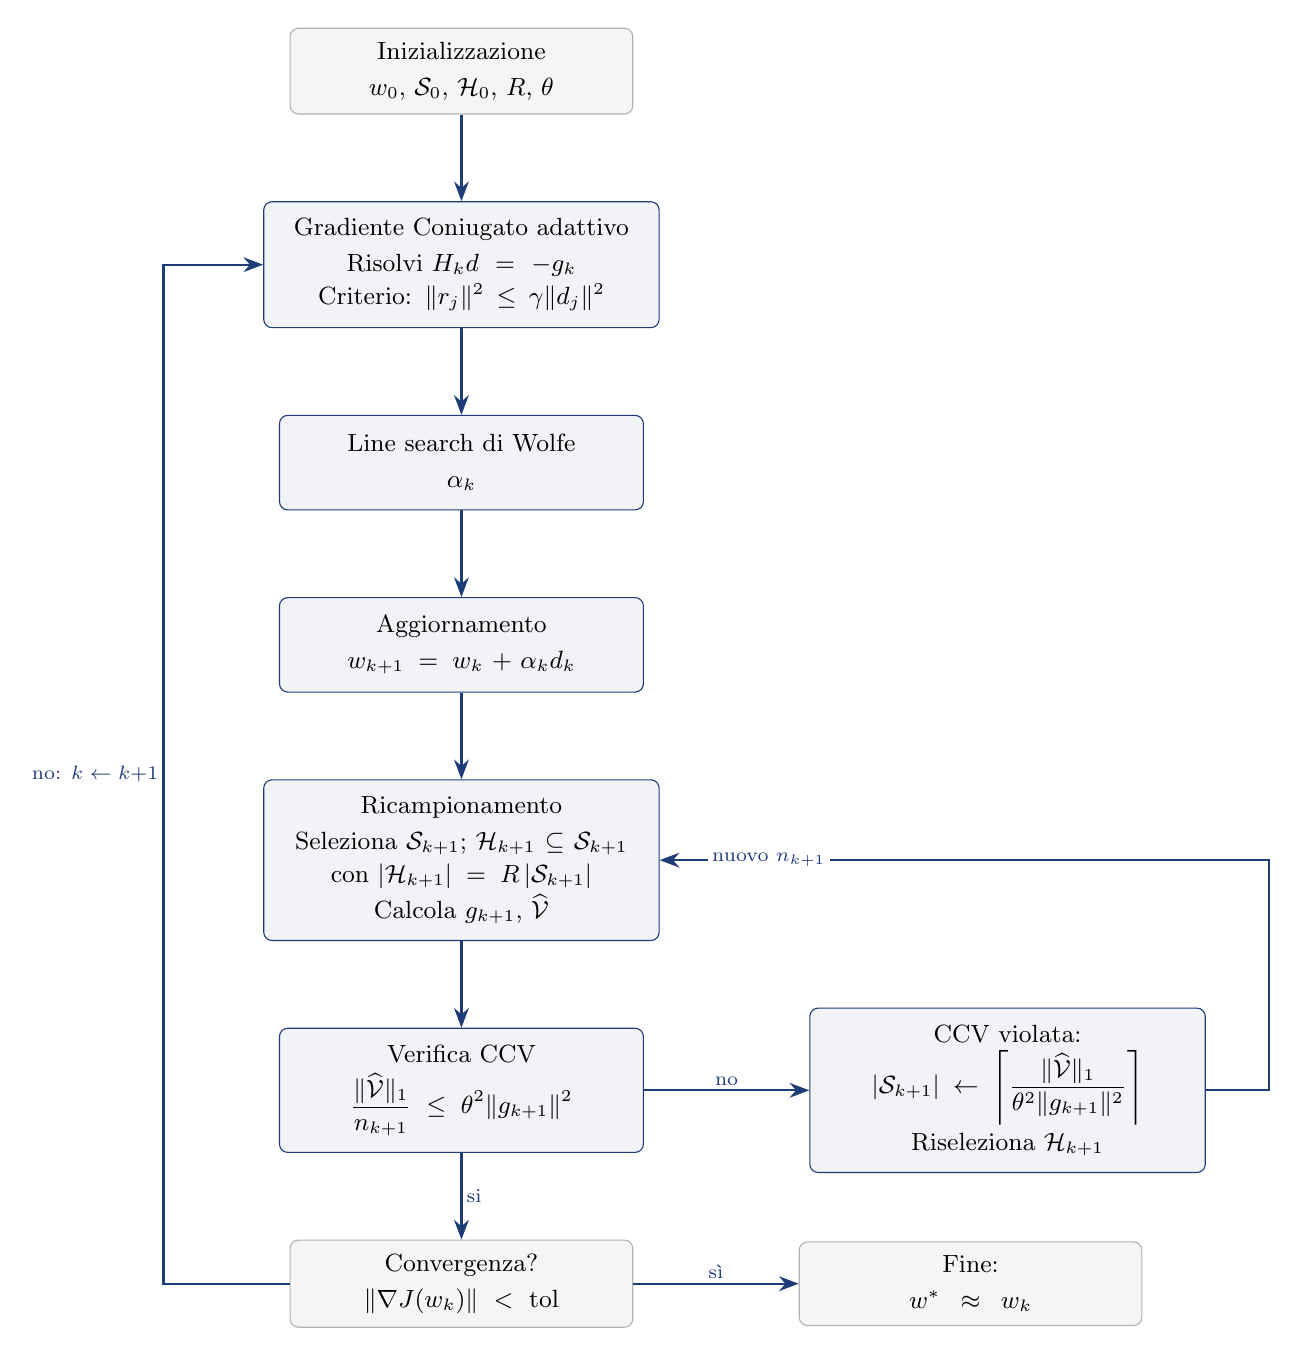
\begin{tikzpicture}[
  node distance=1.1cm and 2.4cm,
  every node/.style={font=\small},
  box/.style={
    draw=coverblue, fill=coverblue!6, rounded corners=3pt,
    text width=4.2cm, align=center, minimum height=1.2cm,
    inner sep=6pt
  },
  io/.style={
    draw=gray!60, fill=gray!8, rounded corners=3pt,
    text width=4.0cm, align=center, minimum height=1.0cm,
    inner sep=5pt
  },
  arrow/.style={-{Stealth[length=2.5mm]}, thick, color=coverblue},
  label/.style={font=\scriptsize, fill=white, inner sep=1.5pt}
]

  % Nodi principali (colonna centrale)
  \node[io] (init) {Inizializzazione\\[2pt] $w_0$, $\mathcal{S}_0$, $\mathcal{H}_0$, $R$, $\theta$};
  \node[box, below=of init, text width=4.6cm, minimum height=1.4cm] (cg) {Gradiente Coniugato adattivo\\[2pt] Risolvi $H_k d = -g_k$\\[1pt] Criterio: $\|r_j\|^2 \le \gamma\|d_j\|^2$};
  \node[box, below=of cg] (ls) {Line search di Wolfe\\[2pt] $\alpha_k$};
  \node[box, below=of ls] (upd) {Aggiornamento\\[2pt] $w_{k+1} = w_k + \alpha_k d_k$};
  \node[box, below=of upd, text width=4.6cm, minimum height=1.4cm] (recamp) {Ricampionamento\\[2pt] Seleziona $\mathcal{S}_{k+1}$; $\mathcal{H}_{k+1}\subseteq\mathcal{S}_{k+1}$\\[1pt] con $|\mathcal{H}_{k+1}| = R\,|\mathcal{S}_{k+1}|$\\[1pt] Calcola $g_{k+1}$, $\widehat{\mathcal{V}}$};
  \node[box, below=of recamp] (ccv) {Verifica CCV\\[3pt] $\displaystyle\frac{\|\widehat{\mathcal{V}}\|_1}{n_{k+1}} \le \theta^2 \|g_{k+1}\|^2$};
  \node[io, below=of ccv] (conv) {Convergenza?\\[2pt] $\|\nabla J(w_k)\| < \mathrm{tol}$};
  \node[io, right=2.1cm of conv] (end) {Fine:\\[2pt] $w^* \approx w_k$};

  % Nodo laterale (aumento batch)
  \node[box, right=2.1cm of ccv, text width=4.6cm, minimum height=1.6cm] (grow) {
    CCV violata:\\[2pt]
    $|\mathcal{S}_{k+1}| \leftarrow \left\lceil \dfrac{\|\widehat{\mathcal{V}}\|_1}{\theta^2 \|g_{k+1}\|^2} \right\rceil$\\[2pt]
    Riseleziona $\mathcal{H}_{k+1}$
  };

  % Frecce verticali principali
  \draw[arrow] (init) -- (cg);
  \draw[arrow] (cg) -- (ls);
  \draw[arrow] (ls) -- (upd);
  \draw[arrow] (upd) -- (recamp);
  \draw[arrow] (recamp) -- (ccv);
  \draw[arrow] (ccv) -- (conv) node[label, midway, right] {si};
  \draw[arrow] (conv) -- (end) node[label, midway, above] {sì};

  % Freccia CCV violata
  \draw[arrow] (ccv) -- (grow) node[label, midway, above] {no};

  % Loop ritorno da grow a recamp (percorso esterno destro)
  \draw[arrow] (grow.east) -- ++(0.8,0) |- ($(recamp.east)+(0.8,0)$) -- (recamp.east)
    node[label, pos=0.25, right] {nuovo $n_{k+1}$};

  % Loop ritorno da conv a cg (percorso esterno sinistro)
  \draw[arrow] (conv.west) -- ++(-1.6,0) |- (cg.west)
    node[label, pos=0.25, left] {no: $k \leftarrow k{+}1$};

\end{tikzpicture}
\end{document}
